When it comes to blackbox attacks, the transfer based approach introduced in Section \ref{sec:transfer-based} is evaluated as well as the boundary attack from Section \ref{sec:boundary-attack}. It is worth mentioning that in this thesis a \textit{blackbox attack} means that the adversary can only query the targeted neural network and obtain an associated label. The adversary has no information about the confidence of the network in the prediction or any kind of list of most probable labels.

In the transfer based approach, as described in Section \ref{sec:transfer-based}, the goal is to train a substitute network that will learn similar decision boundaries for every class as the targeted network. This implies that total number of possible classes must be the same, but an architecture of the substitute network may be different from the architecture of the targeted network.

To get information about boundaries of the targeted neural network,  I take 778 samples that are previously unseen to targeted neural network, obtain labels for those samples and train a substitute neural network based on those results. Distribution of samples over age is presented in Figure \ref{fig:custom-dataset}.
 
 \begin{figure}[h]
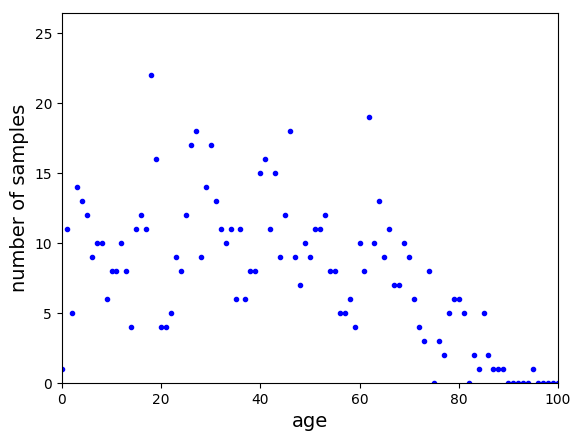
\includegraphics[width=13cm]{custom-dataset}
\caption{Number of samples per age in the dataset that is used for training a substitute neural network by querying a targeted blackbox neural network}
\label{fig:custom-dataset}
\end{figure}

Next, I take random 200 samples that are yet unseen by both networks and evaluate MAE of the targeted neural network and the substitute network on those 200 images. Then I craft adversarial samples for the substitute neural network using those 200 images. Target labels for adversarial samples are set in the same manner as in whitebox attacks, i.e. label 90 if a person is under 50 years old and label 10 if a person is over 50 years old. 

Finally, I evaluate MAE of the targeted neural network and the substitute network on the 200 adversarial samples crafted in the previous step.

In my first attempt, I tried to use the InceptionResNetV2 architecture as a substitute network. However, the experiment failed due to memory consumption when the jacobian augmentation of the dataset is performed. 

In my second attempt, I used ResNet50 architecture for a substitute network instead of InceptionResNetV2 architecture. However, the experiment again failed  due to the memory exhaustion when the jacobian augmentation of the dataset is performed.  

In my third attempt, I used a vanilla CNN with three convolutional layers followed by flatten layer and softmax layer used for classification. However, the experiment failed again due to the same reason..


Finally, I skip the step of the jacobian augmentation of the dataset in the transfer based approach and manage to run the experiments. The jacobian augmentation is a heuristic that computes how to expand the existing dataset so that new samples are closer to boundaries of being classified as a certain class. Instead of using this heuristic, I query once the targeted neural network, train the substitute network based on the associated labels provided by the targeted neural network and execute the attack. This way the substitute network does learn information about classification boundaries of the targeted neural network, but less than it would learn using the jacobian augmentation. Further argumentation of this decision can be found in Section \ref{sec:threats-to-validity}.

Results of this modified transfer based approach are presented in Tables
\ref{table:bbox-resnet50-sgd-fgsm},
\ref{table:bbox-resnet50-adam-fgsm}, 
\ref{table:bbox-resnet50-sgd-cw},
\ref{table:bbox-resnet50-adam-cw}, 
\ref{table:bbox-inception-sgd-fgsm},
\ref{table:bbox-inception-adam-fgsm}, 
\ref{table:bbox-inception-sgd-cw}, and
\ref{table:bbox-inception-adam-cw}.

% Please add the following required packages to your document preamble:
% \usepackage{graphicx}
\begin{table}[]
\resizebox{\textwidth}{!}{%
\begin{tabular}{|c|c|c|c|c|c|c|c|c|}
\hline
 & \multicolumn{2}{c|}{clean samples} & \multicolumn{6}{c|}{adversarial samples} \\ \hline
blackbox model id & blackbox MAE & substitute MAE & blackbox MAE & substitute MAE & avg L2 & std dev L2 & min L2 & max L2 \\ \hline
1 &  6.42 &  12.42 & 6.92 & 19.14  &  1890.86 & 58.77 &  1580.84 & 1939.89 \\ \hline
2 & 6.99 & 11.52 & 10.2 &  23.145 &  1891.01 & 59.07 & 1565.25 & 1939.89  \\ \hline
3 & 5.29 & 14.275 & 5.79  & 25.685 & 1891.34  & 58.79 & 1559.34 & 1939.89  \\ \hline
4 & TODO & TODO & TODO & TODO &  TODO & TODO & TODO &  \\ \hline
\end{tabular}%
}
\caption{Substitute network: ResNet50 architecture with SGD optimizer; Attack: FGSM}
\label{table:bbox-resnet50-sgd-fgsm}
\end{table}

% Please add the following required packages to your document preamble:
% \usepackage{graphicx}
\begin{table}[]
\resizebox{\textwidth}{!}{%
\begin{tabular}{|c|c|c|c|c|c|c|c|c|}
\hline
 & \multicolumn{2}{c|}{clean samples} & \multicolumn{6}{c|}{adversarial samples} \\ \hline
blackbox model id & blackbox MAE & substitute MAE & blackbox MAE & substitute MAE & avg L2 & std dev L2 & min L2 & max L2 \\ \hline
1 & 6.42 & 20.275 & 6.99 & 19.91  & 1890.10 & 60.31  &  1555.87 & 1939.89  \\ \hline
2 & 6.99 & 11.94 & 7.44 & 12.145 & 1921.91  &  21.20 &  1809.24 & 1939.89  \\ \hline
3 & 5.29 & 24.99 & 26.1 & 4.91 & 1893.30 & 58.41 & 1534.87 & 1939.89  \\ \hline
4 &  &  &  &  &  &  &  &  \\ \hline
\end{tabular}%
}
\caption{Substitute network: ResNet50 architecture with Adam optimizer; Attack: FGSM}
\label{table:bbox-resnet50-adam-fgsm}
\end{table}

% Please add the following required packages to your document preamble:
% \usepackage{graphicx}
\begin{table}[]
\resizebox{\textwidth}{!}{%
\begin{tabular}{|c|c|c|c|c|c|c|c|c|}
\hline
 & \multicolumn{2}{c|}{clean samples} & \multicolumn{6}{c|}{adversarial samples} \\ \hline
blackbox model id & blackbox MAE & substitute MAE & blackbox MAE & substitute MAE & avg L2 & std dev L2 & min L2 & max L2 \\ \hline
1 & 6.42 &  13.73 & 6.17 & 14.90 & 369.75 & 1407.87  & 0.0  & 6269.29 \\ \hline
2 & 6.99 & 9.54  & 6.99 &  9.54 & 0.00 & 0.00 & 0.00 & 0.00 \\ \hline
3 & 5.29 &  &  &  &  &  &  &  \\ \hline
4 &  &  &  &  &  &  &  &  \\ \hline
\end{tabular}%
}
\caption{Substitute network: ResNet50 architecture with SGD optimizer; Attack: CW}
\label{table:bbox-resnet50-sgd-cw}
\end{table}

% Please add the following required packages to your document preamble:
% \usepackage{graphicx}
\begin{table}[]
\resizebox{\textwidth}{!}{%
\begin{tabular}{|c|c|c|c|c|c|c|c|c|}
\hline
 & \multicolumn{2}{c|}{clean samples} & \multicolumn{6}{c|}{adversarial samples} \\ \hline
blackbox model id & blackbox MAE & substitute MAE & blackbox MAE & substitute MAE & avg L2 & std dev L2 & min L2 & max L2 \\ \hline
1 & 6.42 & 17.45 & 6.42 & 17.45  & 0.00 & 0.00  & 0.00 & 0.00 \\ \hline
2 & 6.99 & 10.53 & 6.99 & 10.53  & 0.00 & 0.00 & 0.00  & 0.00 \\ \hline
3 & 5.29 &  &  &  &  &  &  &  \\ \hline
4 &  &  &  &  &  &  &  &  \\ \hline
\end{tabular}%
}
\caption{Substitute network: ResNet50 architecture with Adam optimizer; Attack: CW}
\label{table:bbox-resnet50-adam-cw}
\end{table}

% Please add the following required packages to your document preamble:
% \usepackage{graphicx}
\begin{table}[]
\resizebox{\textwidth}{!}{%
\begin{tabular}{|c|c|c|c|c|c|c|c|c|}
\hline
 & \multicolumn{2}{c|}{clean samples} & \multicolumn{6}{c|}{adversarial samples} \\ \hline
blackbox model id & blackbox MAE & substitute MAE & blackbox MAE & substitute MAE & avg L2 & std dev L2 & min L2 & max L2 \\ \hline
1 & 6.42 & 10.20 & 7.57 & 13.63 & 2524.84 & 77.62 & 2097.67 & 2589.41 \\ \hline
2 & 6.99  & 11.09 & 10.66  &  18.59 & 2525.10 & 76.92 & 2105.15 & 2589.41 \\ \hline
3 & 5.29 & 21.015 & 5.57 & 25.09 & 2527.32 & 73.56 & 2143.89 & 2589.41  \\ \hline
4 &  &  &  &  &  &  &  &  \\ \hline
\end{tabular}%
}
\caption{Substitute network: InceptionResNetV2 architecture with SGD optimizer; Attack: FGSM}
\label{table:bbox-inception-sgd-fgsm}
\end{table}

% Please add the following required packages to your document preamble:
% \usepackage{graphicx}
\begin{table}[]
\resizebox{\textwidth}{!}{%
\begin{tabular}{|c|c|c|c|c|c|c|c|c|}
\hline
 & \multicolumn{2}{c|}{clean samples} & \multicolumn{6}{c|}{adversarial samples} \\ \hline
blackbox model id & blackbox MAE & substitute MAE & blackbox MAE & substitute MAE & avg L2 & std dev L2 & min L2 & max L2 \\ \hline
1 & 6.42 &  &  &  &  &  &  &  \\ \hline
2 & 6.99 &  &  &  &  &  &  &  \\ \hline
3 & 5.29 &  &  &  &  &  &  &  \\ \hline
4 &  &  &  &  &  &  &  &  \\ \hline
\end{tabular}%
}
\caption{Substitute network: InceptionResNetV2 architecture with Adam optimizer; Attack: FGSM}
\label{table:bbox-inception-adam-fgsm}
\end{table}

% Please add the following required packages to your document preamble:
% \usepackage{graphicx}
\begin{table}[]
\resizebox{\textwidth}{!}{%
\begin{tabular}{|c|c|c|c|c|c|c|c|c|}
\hline
 & \multicolumn{2}{c|}{clean samples} & \multicolumn{6}{c|}{adversarial samples} \\ \hline
blackbox model id & blackbox MAE & substitute MAE & blackbox MAE & substitute MAE & avg L2 & std dev L2 & min L2 & max L2 \\ \hline
1 & 6.42 & 18.55 & 6.42 &  18.55 & 0.00 &  & 0.00 & 0.00  \\ \hline
2 & 6.99  & 14.82 &  &  &  &  &  &  \\ \hline
3 & 5.29  &  &  &  &  &  &  &  \\ \hline
4 &  &  &  &  &  &  &  &  \\ \hline
\end{tabular}%
}
\caption{Substitute network: InceptionResNetV2 architecture with SGD optimizer; Attack: CW}
\label{table:bbox-inception-sgd-cw}
\end{table}

% Please add the following required packages to your document preamble:
% \usepackage{graphicx}
\begin{table}[]
\resizebox{\textwidth}{!}{%
\begin{tabular}{|c|c|c|c|c|c|c|c|c|}
\hline
 & \multicolumn{2}{c|}{clean samples} & \multicolumn{6}{c|}{adversarial samples} \\ \hline
blackbox model id & blackbox MAE & substitute MAE & blackbox MAE & substitute MAE & avg L2 & std dev L2 & min L2 & max L2 \\ \hline
1 & 6.42 &  &  &  &  &  &  &  \\ \hline
2 & 6.99 &  &  &  &  &  &  &  \\ \hline
3 & 5.29 &  &  &  &  &  &  &  \\ \hline
4 &  &  &  &  &  &  &  &  \\ \hline
\end{tabular}%
}
\caption{Substitute network: InceptionResNetV2 architecture with Adam optimizer; Attack: CW}
\label{table:bbox-inception-adam-cw}
\end{table}

Regarding the boundary attack, it's hard to do any quantitative analysis because the attack, as described in Section \ref{sec:boundary-attack}, is fundamentally different than the transfer based approach. 

One sample can be seen in Figure \ref{fig:trump-adv} and the corresponding results in Figure \ref{fig:trump-softmax}. It is interesting to observe what is happening during the attack. 

In the beginning of the attack, as presented in Figure \ref{fig:starting-image-softmax}, the original sample is classified as 68 years old and the targeted image, as presented in Figure \ref{fig:targeted-image-softmax}, is classified as 4 years old. 

As the attack performs more queries, the adversarial sample is looking more and more like the targeted image, but the values that the network is predicting also start to correspond to the targeted image. This can be seen in Figure \ref{fig:trump-softmax}.

Finally when the attack is finished, the adversarial sample seems as the targeted image and the network is very aware of it, i.e. there is a high probability that the adversarial sample is classified as 4 years old. However, probability that the person in the adversarial image is 68 years old is just a bit higher than the probability that the person is 4 years old and that is enough for the network to classify the person as 68 years old. 

\begin{figure}
\begin{subfigure}{.5\textwidth}
  \centering%
  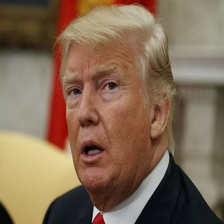
\includegraphics[height=5cm, width=\linewidth, keepaspectratio]{image0.jpg}
  \caption{The starting image}
\end{subfigure}
\begin{subfigure}{.5\textwidth}
  \centering
  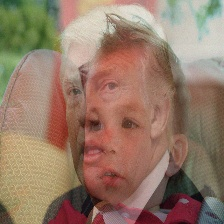
\includegraphics[height=5cm, width=\linewidth, keepaspectratio]{image1000.jpg}
  \caption{1000 queries}
\end{subfigure}

\begin{subfigure}{.5\textwidth}
  \centering
  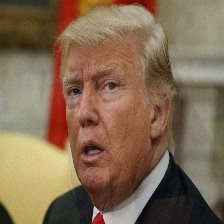
\includegraphics[height=5cm, width=\linewidth, keepaspectratio]{image2000.jpg}
  \caption{2000 queries}
\end{subfigure}
\begin{subfigure}{.5\textwidth}
  \centering
  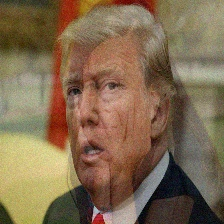
\includegraphics[height=5cm, width=\linewidth, keepaspectratio]{image4000.jpg}
  \caption{4000 queries}
\end{subfigure}

\begin{subfigure}{.5\textwidth}
  \centering
  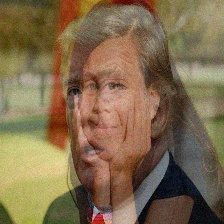
\includegraphics[height=5cm, width=\linewidth, keepaspectratio]{image8000.jpg}
  \caption{8000 queries}
\end{subfigure}
\begin{subfigure}{.5\textwidth}
  \centering
  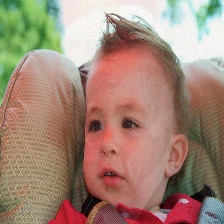
\includegraphics[height=5cm, width=\linewidth, keepaspectratio]{image12000.jpg}
  \caption{12000 queries}
\end{subfigure}

\begin{subfigure}{.5\textwidth}
  \centering
  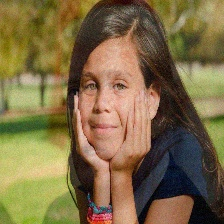
\includegraphics[height=5cm, width=\linewidth, keepaspectratio]{image16000.jpg}
  \caption{16000 queries}
\end{subfigure}
\begin{subfigure}{.5\textwidth}
  \centering
  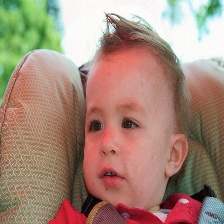
\includegraphics[height=5cm, width=\linewidth, keepaspectratio]{final_adversarial.jpg}
  \caption{Final adversarial sample}
\end{subfigure}
\caption{Although an adversary is changing the image, the blackbox classifier is not changing the prediction (68 years old)}
\label{fig:trump-adv}
\end{figure}

\begin{figure}
\begin{subfigure}{.5\textwidth}
  \centering
  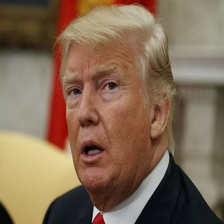
\includegraphics[height=5cm, width=\linewidth, keepaspectratio]{image0.jpg}
  \caption{Starting image}
\end{subfigure}
\begin{subfigure}{.5\textwidth}
  \centering
  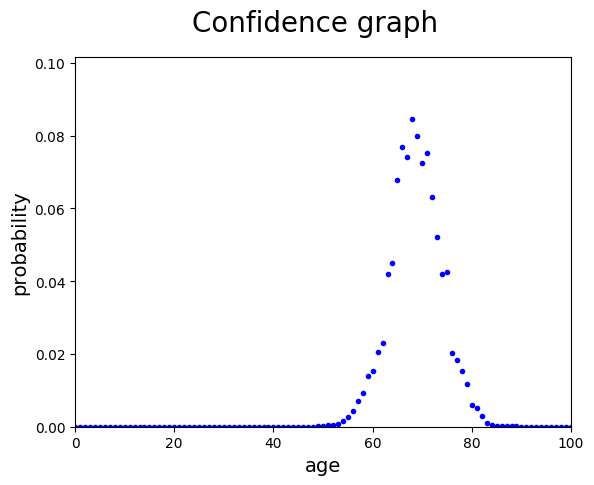
\includegraphics[height=5cm, width=\linewidth, keepaspectratio]{softmaxbenign.png}
  \caption{Predictions for the starting image}
\end{subfigure}
\caption{Starting image and the corresponding prediction}
\label{fig:starting-image-softmax}
\end{figure}

\begin{figure}
\begin{subfigure}{.5\textwidth}
  \centering
  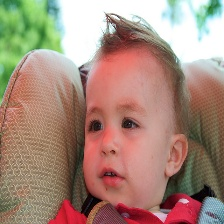
\includegraphics[height=5cm, width=\linewidth, keepaspectratio]{source_image.jpg}
  \caption{The targeted image}
\end{subfigure}
\begin{subfigure}{.5\textwidth}
  \centering
  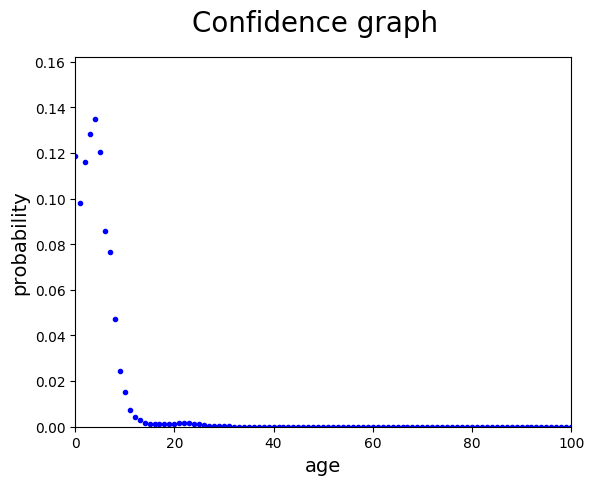
\includegraphics[height=5cm, width=\linewidth, keepaspectratio]{softmaxsource_image.png}
  \caption{Predictions for the targeted image}
\end{subfigure}

\caption{Targeted image and the corresponding predictions}
\label{fig:targeted-image-softmax}
\end{figure}

\begin{figure}

\begin{subfigure}{.5\textwidth}
  \centering%
  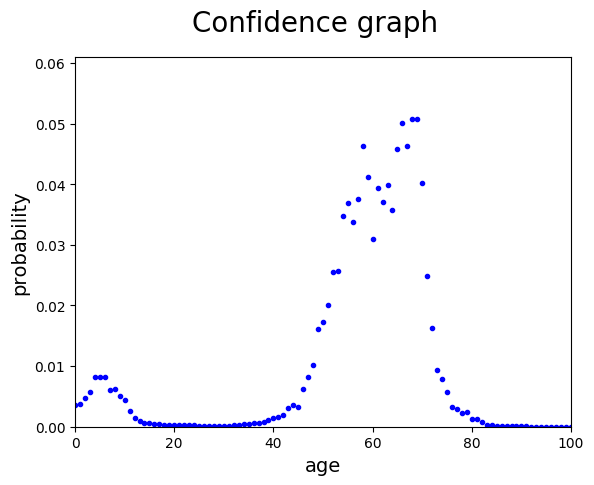
\includegraphics[height=5cm, width=\linewidth, keepaspectratio]{softmax3000.png}
  \caption{3000 queries}
\end{subfigure}
\begin{subfigure}{.5\textwidth}
  \centering%
  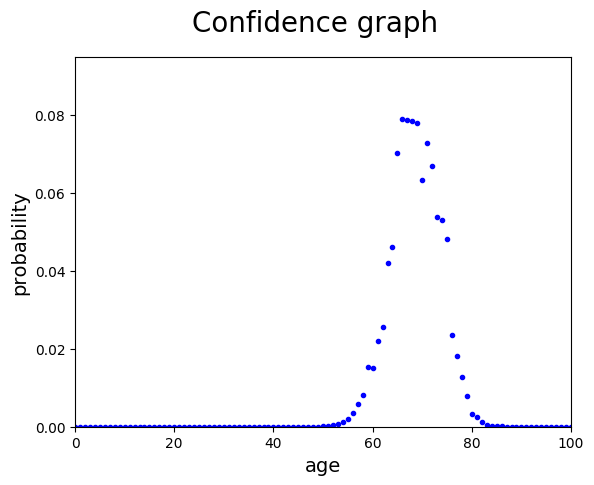
\includegraphics[height=5cm, width=\linewidth, keepaspectratio]{softmax4000.png}
  \caption{4000 queries}
\end{subfigure}


\begin{subfigure}{.5\textwidth}
  \centering%
  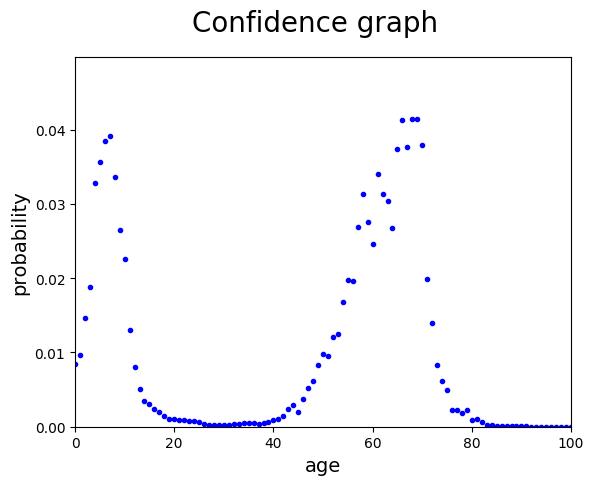
\includegraphics[height=5cm, width=\linewidth, keepaspectratio]{softmax8000.png}
  \caption{8000 queries}
\end{subfigure}
\begin{subfigure}{.5\textwidth}
  \centering%
  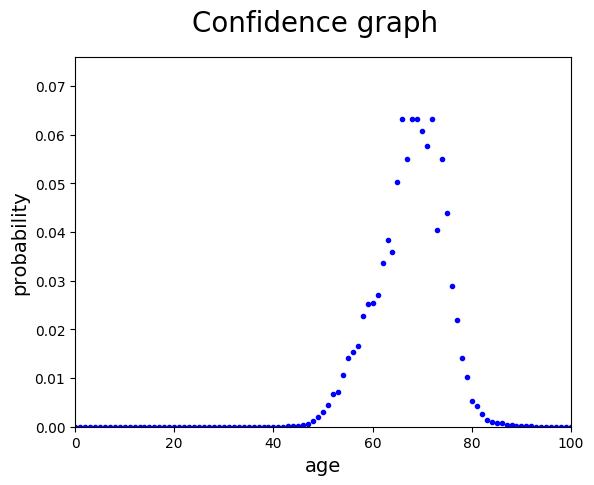
\includegraphics[height=5cm, width=\linewidth, keepaspectratio]{softmaxadversarial.png}
  \caption{The final adversarial sample (77 000 queries)}
\end{subfigure}

\caption{Predictions of the blackbox classifier for images corresponding to Figure \ref{fig:trump-adv}. In all the graphs, age 68 is predicted with the maximum probability.}
\label{fig:trump-softmax}
\end{figure}


